\documentclass[10pt]{article}
\usepackage[utf8]{inputenc}
\usepackage{geometry}
\usepackage[sort]{natbib}
\usepackage{pxfonts}
\usepackage{graphicx}
\usepackage{setspace}
\usepackage{hyperref}
\usepackage{lineno}
\usepackage{authblk}

\doublespacing
\linenumbers


\title{Fitness tracking reveals task-specific associations between
  memory, mental health, and exercise}
\author[1, $\star$]{Jeremy R. Manning}
\author[1,2]{Gina M. Notaro}
\author[1]{Esme Chen}
\author[1]{Paxton C. Fitzpatrick}
\affil[1]{Dartmouth College, Hanover, NH}
\affil[2]{Lockheed Martin, Bethesda, MD}
\affil[$\star$]{Address correspondence to jeremy.r.manning@dartmouth.edu}

\begin{document}
\maketitle

\begin{abstract}
  Physical exercise can benefit both physical and mental well-being.
  Different forms of exercise (i.e., aerobic versus anaerobic; running
  versus walking versus swimming versus yoga; high-intensity interval
  training versus endurance workouts; etc.) impact physical fitness
  in different ways.  For example, running may substantially impact
  leg and heart strength but only moderately impact arm strength. We
  hypothesized that the mental benefits of exercise might be similarly
  differentiated.  We focused specifically on how different forms of
  exercise might related to different aspects of memory and mental
  health.  To test our hypothesis, we collected nearly a century's
  worth of fitness data (in aggregate).  We then asked participants to
  fill out surveys asking them to self-report on different aspects of
  their mental health.  We also asked participants to engage in a
  battery of memory tasks that tested their short and long term
  episodic, semantic, and spatial memory.  We found that participants
  with similar exercise habits and fitness profiles tended to also
  exhibit similar mental health and task performance profiles.
\end{abstract}

\section*{Introduction}
Engaging in physical activity (exercise) can improve our physical
fitness by increasing muscle strength~\citep{RogeEvan93, Lind79,
  CranEtal13, Knut07}, increasing bone density~\citep{ChilEtal12,
  BassRams94, LaynNels99}, increasing cardiovascular
performance~\citep{MaioEtal00, PollEtal00}, increasing lung
capacity~\citep{LazoEtal16}~\citep[although see][]{RomaEtal16},
increasing endurance~\citep{WilmKnut03}, and more.  Exercise can also
improve mental health~\citep{Ragl90, MikkEtal17, TaylEtal85,
  DeslEtal09, Call04, PaluSchw00, BassSuzu17} and cognitive performance~\citep{ChanEtal12b,
  BrisEtal02, EtniEtal06, BassSuzu17}.

The physical benefits of exercise can be explained by stress-responses
of the affected body tissues. For example, skeletal muscles that are
taxed during exercise exhibit stress responses~\citep{MortEtal09} that
can in turn affect their growth or atrophy~\citep{SchiEtal13}.  By
comparison, the benefits of exercise on mental health are less direct.  For
example, one hypothesis is that exercise leads to specific
physiological changes, such as increased aminergic synaptic
transmission and endorphin release, which in turn act on
neurotransmitters in the brain~\citep{PaluSchw00}.

Speculatively, if different exercise regimens lead to different
neurophysiological responses, one might be able to map out a spectrum
of signalling and transduction pathways that are impacted by a given
type, duration, and intensity of exercise in each brain region.  For
example, prior work has shown that exercise increases acetylcholine
levels, starting in the vicinity of the exercised
muscles~\citep{ShoeEtal97}.  Acetylcholine is thought to play an
important role in memory formation~\citep[e.g., by modulating specific
synaptic inputs from entorhinal cortex to the hippocampus, albeit in
rodents;]{PalaEtal21}.  Given the central role of these medial
temporal lobe structures play in memory, changes in acetylcholine
might lead to specific changes in memory formation and retrieval.

In the present study, we hypothesize that (a) different exercise regimens will
have different, quantifiable impacts on cognitive performance and
mental health, and that (b) these impacts will be consistant across
individuals.  To this end, we collected a year of fitness tracking
data from each of 113 participants.  We then asked each participant to
fill out a brief survey in which they self-evaluated several aspects
of their mental health.  Finally, we ran each participant through a
battery of memory tasks, which we used to evaluate their memory
performance along several dimensions.  We examined the data for
potential associations between memory, mental health, and exercise.

\section*{Results}
\begin{itemize}
\item characterizing behaviors (potentially broken down by 3--4
  fitness-defined categories, like activity level quartile; may also
  want to have separate figures: one for characterizing behaviors on
  average, and a second breaking down by fitness variable, e.g. after
  the correlation analyses are presented)
  \begin{itemize}
  \item Free recall: pfr, lag-CRP, spc
    \item Naturalistic recall: reproduce a version of the sherlock
      movie/recall trajectories
    \item Foreign language flashcards: p(correct) by activity level
      \item Spatial learning: mean error by number of shapes
      \end{itemize}
    \item Fitness info (break down by task performance, potentiall
      separately for each task); also separate out recent (raw) and recent versus baseline
      \begin{itemize}
      \item activity (steps, zone minutes, floors/elevation)
      \item resting heart rate
        \item sleep
        \end{itemize}
  \item exploratory analysis (correlations)
    \begin{itemize}
    \item Memory-memory
    \item fitness-fitness
    \item survey-survey
    \item (fitness + survey)-memory
    \end{itemize}
  \item predictive analysis (regressions)
    \begin{itemize}
    \item Predict memory performance on held-out task from other tasks
    \item Predict memory performance on each task using fitness data
      \item Predict memory performance on each task using survey data
      \end{itemize}
    \item Reverse correlations: look at recent changes versus baseline trends
      \begin{itemize}
      \item Fitness profile that predicts performance on each task (barplots + timelines)
      \item Fitness profile for each survey demographic (barplots + timelines)
        \begin{itemize}
          \item Select out mental health demographics (based on meds, stress levels)
          \end{itemize}
        \end{itemize}
  \end{itemize}

  \section*{Discussion}
  \begin{itemize}
  \item summarize key findings
  \item correlation versus causation
         \item what can vs. can't we know?  we can identify correlations, but not causal direction-- e.g. we cannot know whether exercise \textit{causes} mental changes versus whether people with particular neural profiles might tend to engage in particular exercise behaviors.  that being said, we \textit{can} separate out baseline tendencies (e.g., how people tend to exercise in general) versus recent changes (e.g., how they happened to have exercised prior to the experiment).
  \item related work (exercise/memory, exercise/mental health), what this study adds
    \item future direction: towards customized physical exercise recommendation engine for optimizing mental health and mental fitness
    \end{itemize}

    \section*{Methods}

    We ran an online experiment using the Amazon Mechanical Turk
    platform.  We collected data about each participant's fitness and
    exercise habits, a variety of self-reported measures concerning their
    mental health, and about their performance on a battery of memory
    tasks.  We mined the dataset for potential associations between
    memory, mental health, and exercise.

    
    
\subsection*{Experiment}
\subsubsection*{Participants}
We recruited experimental participants by posting our experiment as a
Human Intelligence Task (HIT) on the Amazon Mechanical Turk platform.
We limited participation to Mechanical Turk Workers who had been
assigned a ``Masters'' designation on the platform, given to workers
who score highly across several metrics on a large number of HITs,
according to a proprietary algorithm managed by Amazon.  We further
limited our participant pool to participants who self-reported that
they were fluent in English and regularly used a Fitbit fitness
tracker device.  A total of 160 workers accepted our
HIT in order to participate in our experiment.  Of these, we excluded all
participants who failed to log into their Fitbit account (giving us
access to their anonymized fitness tracking data), encountered
technical issues (e.g., by accessing the HIT using an incompatible browser, device, or
operating system), or who ended their participation prematurely,
before completing the full study.  In all, 113 participants remained
that contributed usable data to the study.

For their participation, workers received a base payment of \$5 per hour (computed in 15
minute increments, rounded up to the nearest 15 minutes), plus an
additional performance-based bonus of up to \$5.  Our recruitment
procedure and study protocol
were approved by Dartmouth's Committee for the Protection of Human Subjects.

\paragraph{Gender, age, and race.}
Of the 113 participants who contributed usable data, 77 reported their gender as female, 35 as
male, and 1 chose not to report their gender.  Participants ranged in
age from 19--68 years old (25\textsuperscript{th} percentile: 28.25
years; 50\textsuperscript{th} percentile: 32 years;
75\textsuperscript{th} percentile: 38 years).  Participants reported
their race as White (90 participants), Black or African American (11
participants), Asian (7 participants), Other (4 participants), and
American Indian or Alaska Native (3 participants).  One participant
opted not to report their race.

\paragraph{Languages.}
All participants reported that they were fluent in either 1 and 2
languages (25\textsuperscript{th} percentile: 1;
50\textsuperscript{th} percentile: 1; 75\textsuperscript{th}
percentile: 1), and that they were ``familiar'' with between 1 and 11
languages (25\textsuperscript{th} percentile: 1;
50\textsuperscript{th} percentile: 2; 75\textsuperscript{th}
percentile: 3).

\paragraph{Reported medical conditions and medications.}
Participants reported having and/or taking medications pertaining to the following medical conditions: anxiety or
depression (4 participants), recent head injury (2 participants), high
blood pressure (1 participant), bipolar (1 participant),
hypothyroidism (1 participant), and other unspecified medications (1
participant).  Participants reported their current and typical stress
levels on a Likert scale as very relaxed (-2), a little relaxed (-1),
neutral (0), a little stressed (1), or very stressed (2).  The
``current'' stress level reflected participants' stress at the time
they participated in the experiment.
Their responses
ranged from -2 to 2 (current stress: 25\textsuperscript{th} percentile: -2;
50\textsuperscript{th} percentile: -1; 75\textsuperscript{th}
percentile: 1; typical stress: 25\textsuperscript{th} percentile: 0;
50\textsuperscript{th} percentile: 1; 75\textsuperscript{th}
percentile: 1).  Participants also reported their current level of
alertness on a Likert scale as very sluggish (-2), a little sluggish
(-1), neutral (0), a little alert (1), or very alert (2).  Their
responses ranged from -2 to 2 (25\textsuperscript{th} percentile: 0;
50\textsuperscript{th} percentile: 1; 75\textsuperscript{th}
percentile: 2).  Nearly all (111 out of 113) participants reported
that they had normal color vision, and 15 participants reported
uncorrected visual impairments (including dyslexia and uncorrected
near- or far-sightedness).

\paragraph{Residence and level of education.}
Participants reported their residence
as being located in the suburbs (36 participants), a large city (30
participants), a small city (23 participants), rural (14
participants), or a small town (10 participants).  Participants
reported their level of education as follows: College graduate (42
participants), Master's degree (23 participants), Some college (21
participants), High school graduate (9 participants), Associate's
degree (8 participants), Other graduate or professional school (5
participants), Some graduate training (3 participants), or Doctorate
(2 participants).

\paragraph{Reported water and coffee intake.}
Participants reported the number of cups of water and coffee they had
consumed prior to accepting the HIT.  Water consumption ranged from
0--6 cups (25\textsuperscript{th} percentile: 1;
50\textsuperscript{th} percentile: 3; 75\textsuperscript{th}
percentile: 4).  Coffee consumption ranged from 0--4 cups (25\textsuperscript{th} percentile: 0;
50\textsuperscript{th} percentile: 1; 75\textsuperscript{th}
percentile: 2).


\subsubsection*{Tasks}
Upon accepting the HIT posted on Mechanical Turk, the worker was
directed to read and fill out a screening and consent form, and to
share access to their anonymized Fitbit data via their Fitbit account.
After consenting to participant and successfully sharing their Fitbit
data, participants filled out a survey and then engaged in a series of
memory tasks (Fig.~\ref{fig:tasks}).  All stimuli and code for running
the full Mechanical Turk experiment may be found
\href{https://github.com/ContextLab/brainfit-task}{\underline{here}}.

\begin{figure}[tp]
\centering
\includegraphics[width=1\textwidth]{figs/experiment}
\caption{\textbf{Battery of memory tasks.}  \textbf{a.  Free recall.}
Participants study 16 words (presented one at a time), followed by an
immediate memory test where they type
each word they remember from the just-studied list.  In the delayed
memory test, participants type any words they remember studying, from
any list.  \textbf{b. Naturalistic recall.}  Participants watch a
brief video, followed by two immediate memory tests.  The first test
asks participants to write out what happened in the video.  The second
test has participants answer a series of multiple choice questions
about the conceptual content of the video.  In the delayed memory
test, participants (again) write out what happened in the video.
\textbf{c. Foreign language flashcards.}  Participants study a
sequence of 10 English-Gailic word pairs, each presented with an
illustration of the given word.  During an immediate memory test,
participants perform a multiple choice test where they select the
Gaelic word that corresponds to the given photograph.  During the
delayed memory test, participants perform a second multiple choice
test, where they select the Gaelic word that corresponds to each of a
new set of photographs.  \textbf{d. Spatial learning.}  In each trial,
participants
study a set of randomly positioned shapes.  Next, the shapes'
positions are altered, and participants are asked to drag the shapes
back to their previous positions.  \textbf{All panels.}  The gray
numbers denote the order in which participants experienced each task
or test.}
\label{fig:tasks}
\end{figure}

\paragraph*{Survey questions.}  We collected the following demographic
information from each participant: their birth year, gender, highest
(academic) degree achieved, race, language fluency, and language
familiarity.  We also collected information about participants'
health and wellness, including about their vision, alertness, stress, sleep, coffee
and water consumption, location of their residence, activity typically
required for their job, and exercise habits.


\paragraph*{Free recall (Fig.~\ref{fig:tasks}a).} 
Participants studied a sequence of four word lists, each comprising 16
words.  After studying each list, participants received an immediate
memory test, whereby they were asked to type (one word at a time) any
words they remembered from the just-studied list, in any order.

Words were presented for 2~s each, in black text on a white
background, followed by a 2~s blank (white) screen.  After the final
2~s pause, participants were given 90~s to type in as many words as
they could remember, in any order.  The memory test was constructed
such that the participant could only see the text of the current word
they were typing; when they pressed any non-letter key, the current
word was submitted and the text box they were typing in was cleared.
This was intended to prevent participants from retroactively editing
their previous responses.

The word lists participants studied were drawn from the categorized
lists reported in \cite{ZimaEtal18}.  Each participant was assigned
four unique randomly chosen lists (in a randomized order), selected from a full set of 16
lists.  Each chosen list was then randomly shuffled before presenting
the words to the participants.

Participants also performed a final delayed memory test where they
were given 180~s to type out any words they remembered from
\textit{any} of the 4 lists they had studied.

Recalled words within an edit distance of 2 (i.e., a Levenshtein Distance less
than or equal to 2) of any word in the wordpool were ``autocorrected''
to their nearest match.  We also manually corrected clear typos or
mispellings by hand (e.g., we corrected ``hippoptumas'' to
``hippopotamus'', ``zucinni'' to ``zucchini'', and so on).  Finally,
we lemmatized each submitted word to match the plurality of the
matching wordpool word (e.g., ``bongo'' was corrected to ``bongos'',
and so on).  After applying these corrections, any submitted words
that matched words presented on the just-studied list were tagged as
``correct'' recalls, and any non-matching words were discarded as
``errors.''  Because participants were not allowed to edit the text
they entered, we chose not to analyze these putative ``errors,'' since
we could not distinguish typos from true misrememberings.

\paragraph*{Naturalistic recall (Fig.~\ref{fig:tasks}b).}
Participants watched a 2.5~minute video clip entitled ``The Temple of
Knowledge.''  The video comprises an animated story told to StoryCorps
by Ronald Clark, who was interviewed by his daughter, Jamilah Clark.
The narrator (Ronald) discusses growing up living in an apartment over Washington
Heights branch of the New York Public Library, where his father worked
as a custodian during the 1940s.

After watching the video clip, participants were asked to type out
anything they remembered about what happened in the video.  They typed
their responses into a text box, one sentence at a time.  When the
participant pressed the return key or typed any final punctuation mark
(``.'', ``!'', or ``?'') the text currently entered into the box was
``submitted'' and added to their transcript, and the text box was
cleared to prevent further editing of any already-submitted text.
This was intended to prevent participants from retroactively editing
their previous responses.  Participants were given up to 10~minutes to
enter their responses.  After 4~minutes participants were given the
option of ending the response period early, e.g., if they felt they had finished
entering all of the information they remembered.  Each participant's
transcript was constructed from their submitted responses by combining
the sentences into a single document and removing extraneous
whitespace characters.

Following this 4--10 minute free response period, participants were
given a series of 10 multiple choice questions about the conceptual
content of the story.  All participants received the same questions,
in the same order.

Participants also performed a final delayed memory test, where they
carried out the free response recall task a second time, near the end
of the testing session.  This resulted in a second transcript, for
each participant.

\paragraph*{Foreign language flashcards (Fig.~\ref{fig:tasks}c).}
Participants studied a series of 10 English-Gaelic word pairs in a
randomized order.  We selected the Gaelic language both for its
relatively small number of native speakers and for its dissimilarity
to other commonly spoken languages amongst Mechanical Turk Workers.
We verified (via self report) that all of our participants were fluent in English and
that they were neither fluent nor familiar with Gaelic.

Each word's ``flashcard'' comprised a cartoon
depicting the given word, the English word or phrase in lowercase text (e.g., ``the
boy''), and the Gaelic word or phrase in uppercase text (e.g.,
``BUACHAILL'').   Each
flashcard was displayed for 4~s, followed by a 3~s interval (during
which the screen was cleared) prior to the next flashcard
presentation.

After studying all 10 flashcards, participants were given a multiple
choice memory test where they were shown a series of novel
photographs, each depicting one of the 10 words they had learned.
They were asked to select which (of 4 unique options) Gaelic word went with
the given picture.  The 3 incorrect options were selected at random
(with replacement across trials), and the order in which the choices
appeared to the participant were also randomized.  Each of the 10
words they had learned were tested exactly once.

Participants also performed a final delayed memory test, where they
were given a second set of 10 questions (again, one per word they had
studied).  For this second set of questions participants were prompted
with a new set of novel photographs, and new randomly chosen incorrect
choices for each question.  Each of the 10 original words they had
learned were (again) tested exactly once during this final memory test.



\paragraph*{Spatial learning (Fig.~\ref{fig:tasks}d).}
Participants performed a series of study-test trials where they
memorized the onscreen spatial locations of two or more shapes.
During the study phrase of each trial, a set of shapes appeared on the screen for
10~s, followed by 2~s of blank (white) screen.  During the test phase
of each trial, the same shapes appeared onscreen again, but this time
they were vertically aligned and sorted horizontally in a random
order.  Participants were instructed to drag (using the mouse) each
shape to its studied position, and then to click a button to indicate
that the placements were complete.

In different study-test trials, participants learned the locations of
different numbers of shapes (always drawn from the same pool of 7
unique shapes, where each shape appeared at most one time per trial).
They first performed three trials where they learned the locations of
2 shapes; next three trials where they learned the locations of 3
shapes; and so on until their last three trials, where (during each trial) they learned
the locations of 7 shapes.  All told, each participant performed 18
study-test trials of this spatial learning task (3 trials for each of 2, 3,
4, 5, 6, and 7 shapes).


\subsubsection*{Fitness tracking using Fitbit devices}


\begin{figure}[t]
\centering
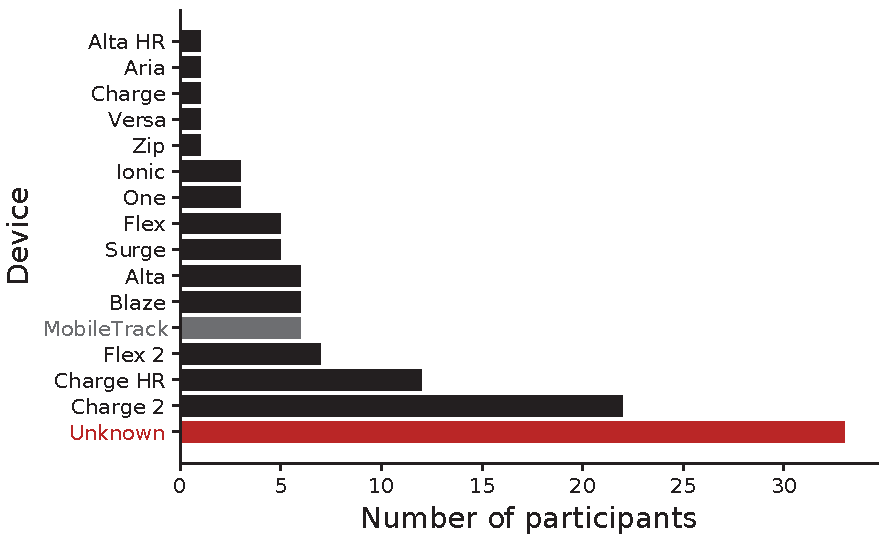
\includegraphics[width=0.6\textwidth]{figs/devices}
\caption{\textbf{Fitbit devices.}  The bars indicate the numbers of
  participants whose fitness tracking data came from each model of
  Fitbit device.  ``MobileTrack'' refers to participants who used
  smartphone accelerometer information to track their activity via the
  Fitbit smartphone app.
  ``Unknown''  denotes participants whose device information was not
  available from their available Fitbit data.}
\label{fig:devices}
\end{figure}

\subsubsection*{Processing Fitbit data}
\paragraph*{Raw metrics.}
\paragraph*{Comparing recent versus baseline measurements.}

\subsubsection*{Exploratory correlation analyses}
\paragraph*{Imputation and interpolation of missing data.}

\subsubsection*{Regression-based prediction analyses}

\subsubsection*{Reverse correlation analyses}




\section*{Acknowledgements}
We acknowledge useful discussions with David Bucci, Emily Glasser, Andrew Heusser, Abigail Bartolome, Lorie Loeb, Lucy Owen, and Kirsten Ziman.  Our work was supported in part by the Dartmouth Young Minds and Brains initiative.  The content is solely the responsibility of the authors and does not necessarily represent the official views of our supporting organizations.  This paper is dedicated to the memory of David Bucci, who helped to inspire the theoretical foundations of this work.  Dave served as a mentor and colleague on the project prior to his passing.


\section*{Data and code availability}
All analysis code and data used in the present manuscript may be found \href{https://github.com/ContextLab/brainfit-paper}{\underline{here}}.

\section*{Author contributions}
Concept: J.R.M.  Experiment implementation and data collection: G.M.N.
Analyses: G.M.N., E.C., P.C.F., and J.R.M.  Writing: J.R.M.

\section*{Competing interests}
The authors declare no competing interests.

\bibliographystyle{apa}
\bibliography{/Users/jmanning/CDL-bibliography/cdl}
\end{document}
